
\subsection{Tool-Flow}
What are the more concrete steps involved in getting this done?
What does the frontend look like (overview) and what about the backend,
is that mostly LegUp?

\begin{figure}[!t]
\centering
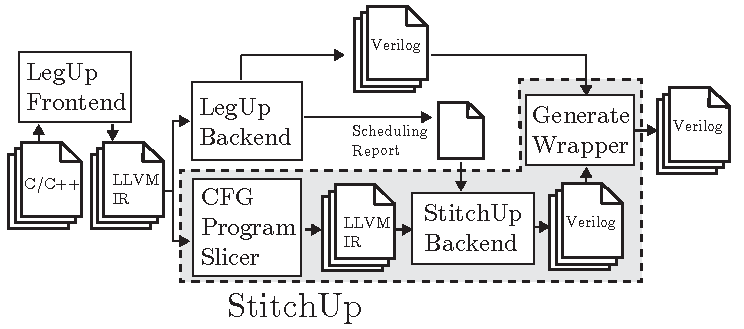
\includegraphics[width=2.5in]{./imgs/tool-flow.pdf}
\caption{Tool Flow Overview diagram}
\label{fig:tool_flow_diagram}
\end{figure}

This section will likely be quite small.

\subsection{Code Analysis Implementation}
What is LLVM? How is the static analysis performed?

\subsection{Code Generation}
What is LegUp? How can this generate StitchUp circuits?
